%\documentclass[11pt]{report}
%\linespread{1.3} %1.3 for one and a half spacing, 1.6 for double
%\usepackage{amsmath, amsthm, amssymb, float, graphicx, caption, subcaption, cite, braket, url,color}
%\usepackage{verbatim}
%
%\usepackage{graphics}
%\usepackage[pdftex]{epsfig}
%\usepackage{epsfig}
%\usepackage{epstopdf}
%
%%\usepackage[nohug,heads=vee]{diagrams}
%%\diagramstyle[labelstyle=\scriptstyle]
%%\graphicspath{{./Figures/}}
%\usepackage[margin=2.5cm]{geometry}
%%\title{Title}
%%\author{Chrysoula Vlachou}
%%\date{}
%\newtheorem{lemma}{Lemma}
%\newtheorem{theorem}{Theorem}
%\newtheorem{proposition}{Proposition}
%%\theoremstyle{definition}
%\newtheorem{definition}{Definition}
%\newtheorem{protocol}{Protocol}
%%\newtheorem*{post}{Postulate}
%%\newtheorem*{rmrk}{Remark}
%%
%\newcommand{\N}{\mathbb N}
%\newcommand{\R}{\mathbb R}
%\newcommand{\C}{\mathbb C}
%\newcommand{\Hilb}{\mathcal H}
%\newcommand{\HRule}{\rule{\linewidth}{0.5mm}}
%\newcommand{\mmobh}{\textlatin{M\"ob}(\mathbb{H})}
%\newcommand{\areah}{\textlatin{area}_{\mathbb{H}}}
%\newcommand{\dth}{d_{\mathbb{H}}}
%\newcommand{\tdth}{$d_{\mathbb{H}}$ }
%\def\h{\mathbb H}
%\DeclareMathOperator{\tr}{Tr}
%\def\I{\hat I}
%\def\ds{\displaystyle}
%\def\ppmod{\!\!\!\!\!\pmod}
%\newcommand{\walkop}{U_{\text{walk}}}
%\newcommand{\proj}[1]{\ket{#1}\bra{#1}}
%\newcommand{\q}[1]{\vec{#1}\cdot\vec{\sigma}}
%
%\def\poly{poly}
%\def\span{span}
%\def\O{\textbf{\textit{O}}}
%\newcommand{\innerproduct}[2]{\langle #1 | #2 \rangle}
%\def\mobh{\textlatin{M\"ob}({\mathbb H})}
%\def\span{span}
%
%
%\begin{document}

\chapter{Simulation of topological systems with quantum walks}

Recently, Kitagawa {\em et al.}~\cite{kit:rud:ber:dem:10} showed that DTQWs can realise topological phases in 1D and 2D for all the symmetry classes~\cite{sch:ryu:fur:lud:08,kit:09} of free-fermion systems. In particular, the authors engineered specific QW protocols that simulate representatives of all topological phases, featured by the presence of robust symmetry-protected edge states (see also~\cite{kit:12}). In general, QW realisations are particularly useful, because, in addition to the simplicity of their mathematical description, the parameters that define them can be easily controlled in the lab. Therefore they provide a powerful simulating platform. The aforementioned topological QWs have been experimentally realised as periodically driven systems~\cite{kit:exp:12} and there are several experimental proposals for measuring topological invariants  employing this approach~\cite{rak:asb:alb:16,gro:bra:alt:mes:asb:16,mug:cel:mas:asb:lew:lob:16}.
In this chapter, we apply the previously introduced fidelity and $\Delta$ analysis of PTs, to the case of the effective Hamiltonians obtained from 1D topological DTQWs, realising representatives of two chiral symmetric classes of TIs.
In particular, we study their topological features at finite temperatures with respect to both single-particle and many-body Boltzmann-Gibbs (BG) thermal-like states.

The chapter is organised as follows: in Section~\ref{sec:top_qw}, we describe the main topological features of QWs and their origin, and present the respective protocols that we use. For a detailed and complete analysis of the topological QW protocols, see~\cite{kit:rud:ber:dem:10,kit:12}. In Section~\ref{sec:density_operators} we present the BG states considered: the single-particle QW states and their many-body counterparts. Furthermore, we clarify the relationship between them and explain the motivation for their use in different physical scenarios. In Section~\ref{sec:results}, we present our results on the fidelity and the quantity $\Delta$ at finite temperatures, and discuss the possibility of temperature-driven PTs. We further confirm these results in Section~\ref{sec:edgeqw}, where we study the behaviour of the edge states. Finally, we summarise and discuss our results and point out possible directions of future work.  
\vfill

\begin{center}
 *The work presented in this chapter corresponds to the work published in~\cite{mer:vla:pau:vie:17:qw}.
\end{center}

\newpage



\section{Topological quantum walks}
\label{sec:top_qw}
In this section, we briefly present the QW protocols that we will use for the simulation of the two chiral symmetric classes BDI and AIII~\cite{sch:ryu:fur:lud:08,kit:09} and describe the origin of their topological features. 
In~\cite{kit:rud:ber:dem:10}, the authors show that the standard DTQW  on the line that we presented in Section~1.4 of Chapter 1, can simulate the non-trivial topological phase of the SSH model for TIs (representative of the BDI symmetry class). In order to be able to study also the trivial topological phase and the edge states, that appear on the boundary between the two, the authors in~\cite{kit:rud:ber:dem:10} introduce the so-called \textit{split-step} QW. As the name suggests, each step of the walk is split in two parts, each having a structure analogous to that of a standard DTQW
\begin{equation}
U_{ss}=T_1R_{y}(\theta_2)T_0R_{y}(\theta_1).
\label{eq:split}
\end{equation}
The coin operators are $R_{y}(\theta_i) = e^{i\frac{\theta_i}{2}\vec{y} \cdot \vec\sigma}$, with $\vec{y}=(0,1,0)$ and $\vec\sigma =(\sigma_x , \sigma_y , \sigma_z)$ the Pauli vector. They represent rotations in the coin space by an angle $\theta_i$ along the $y$-axis, and the shift operators are given as
\begin{equation}
T_{c}=\sum_{x}\ket{x+(-1)^c}\bra{x}\otimes\ket{c}\bra{c}+\ket{x}\bra{x}\otimes\ket{1\oplus c}\bra{1\oplus c},
\end{equation}
where $c\in\{ 0,1\}$ denotes the two possible coin states and $\oplus$ is addition modulo 2.
For different values of the parameters $\theta_1$ and $\theta_2$ this protocol is shown to realise both the trivial and non-trivial topological phases for the SSH model.

As already mentioned, topological QWs can be realised by means of periodically driven systems given by periodic time-dependent Hamiltonians  $H(t+\delta t)=H(t)$, where $\delta t$ represents the time of a single step. The evolution operator for one period of the driving, $[0,\delta t]$, called the Floquet operator, is given by
\begin{equation}
\label{eq:floquet}
U(\delta t)=\mathcal{T}e^{-i\int_{0}^{\delta t}H(t)dt},
\end{equation}
where $\mathcal{T}$ is the time ordering operator. Using homotopy theory, in~\cite{kit:ber:rud:dem:10} the authors propose a classification of periodically driven systems, according to the topological properties of their Floquet operators. They consider the Floquet operator in terms of a local effective Hamiltonian, given by $U(\delta t)=e^{-iH_\text{eff}(\delta t)}$. They show that if $U(\delta t)$ is trivial under all homotopy groups, then the associated $H_\text{eff}$ can exhibit non-trivial topological behaviour. The triviality of $U(\delta t)$ under the homotopy groups implies the existence of a gap in the spectrum of $H_\text{eff}$ and if moreover $H_\text{eff}$ has some of the following symmetries, namely TRS, PHS and  CS, the system supports the topological phases present in static TIs and TSCs, classified according to the system's dimension and the presence of these symmetries~\cite{sch:ryu:fur:lud:08,kit:09}.

The unitary operator that describes one step of the evolution of the split-step QW, as given in Equation~\eqref{eq:split}, is trivial under all homotopy groups, therefore we can define a local effective Hamiltonian 
\begin{equation}
H_{\text{eff}}(\theta_1,\theta_2) \equiv -i\delta t^{-1}\log U(\theta_1,\theta_2), 
\end{equation}
whose quasienergy spectrum has a gap~\cite{kit:ber:rud:dem:10}.
To fix the branch of the logarithm, we choose the first Brillouin zone for the energy spectrum, as in~\cite{asb:12,asb:obu:13}, obtaining the single-particle $H_{\text{eff}}$ consistent with realistic many-body counterparts discussed in the next section. This way, the QW ``provides a stroboscopic simulation of the evolution generated by $H_{\text{eff}}$ at discrete times $N\delta t$''~\cite{kit:rud:ber:dem:10}. In other words, the evolution of the QW is performed in discrete time steps which last $\delta{t}$ units of time each. For simplicity, we take $\delta t=1$.

Writing the effective Hamiltonian as 
\begin{equation}
H_{\text{eff}}(\theta_1,\theta_2) =\sum_{k\in\mathcal{B} }[E_k (\theta_1,\theta_2)\vec{n}_k (\theta_1,\theta_2)\cdot\vec{\sigma}]\otimes\ket{k}\bra{k},
\end{equation}
where $\mathcal {B} $ is the first Brillouin zone, $E_k(\theta_1,\theta_2) \geq 0$ are the eigenvalues and $\vec{n}_k(\theta_1,\theta_2)$ the eigenstates of $H_{\text{eff},k}:$
 \begin{equation}
H_{\text{eff},k} (\theta_1,\theta_2)\ket{\pm\vec{n}_k(\theta_1,\theta_2)} = \pm E_k(\theta_1,\theta_2)\ket{\pm\vec{n}_k(\theta_1,\theta_2)}, 	
\label{Eq: Eigensystem of H_k}
 \end{equation}
forming the two energy bands $\{\pm E_k(\theta_1,\theta_2), \ k\in \mathcal{B}\}$, we can obtain the specific form of the spectrum $E_k(\theta_1,\theta_2)$ and the vectors $\vec{n}_k(\theta_1,\theta_2)$.
 The BDI symmetry class has CS, given by the operator~\cite{kit:rud:ber:dem:10,kit:12} 
 \begin{equation}
 \Gamma_{\theta_1}^y=\exp(-i\pi \vec{A}_{\theta_1}^y\cdot\vec\sigma/2),
 \end{equation}
 where $\vec{A}_{\theta_1}^y=(\cos(\theta_1/2),0,\sin(\theta_1/2))$. 
The CS restricts $\vec{n}_k(\theta_1,\theta_2)$, which defines the quantisation axis for each quasimomentum $k$, to lie on a great circle of the Bloch sphere. The number of times that $\vec{n}_k(\theta_1,\theta_2)$ winds around the origin, as $k$ ranges within the first Brillouin zone $\mathcal B$, is the {\em winding number} $\nu$ of the map between the two circles. This is exactly what manifests the topological features of the QW: the winding number is the topological invariant, whose value characterises each distinct topological phase. Moreover, the BDI class has PHS given by

\begin{equation}
\mathcal{P}=	\mathcal{K},
\end{equation}
where $\mathcal{K}$ denotes the complex conjugation operator, and TRS given by the operator:
\begin{equation}
\mathcal{T}=	\Gamma_{\theta_1}^y\mathcal{P}.
\end{equation}
We can fix $\theta_1=-\pi/2$ for both topological phases, trivial ($\nu=0$) and non-trivial ($\nu=1$). 
The closure of the gap implies a change of phase, so  by varying the value of $\theta_2$ we change the energy spectrum and we are able to close the gap, thus having a PT. 

In order to simulate different symmetry classes, we can further modify this basic split-step protocol. By changing the  rotation axis from $\vec{y}=(0,1,0)$ to $\vec{\alpha}=\frac{1}{\sqrt{2}}(0,1,1)$, we manage to break TRS and PHS, while maintaining CS. That leads us to the split-step protocol that simulates the symmetry class AIII. 
The CS of the AIII class is given by the operator~\cite{kit:rud:ber:dem:10,kit:12} 
\begin{equation}
\Gamma_{\theta_1}^{\alpha}=\exp(-i\pi \vec{A}_{\theta_1}^{\alpha}\cdot\vec\sigma/2),
\end{equation}
where $\vec{A}_{\theta_1}^{\alpha}=(\cos(\theta_1/2),-\frac{1}{\sqrt{2}}\sin(\theta_1/2),\frac{1}{\sqrt{2}}\sin(\theta_1/2))$. Similarly to the case of the BDI class, the existence of CS implies that the vector $\vec{n}_k (\theta_1,\theta_2)$ is restricted to lie on a great circle of the Bloch sphere. The winding number $\nu$ of the map from the first Brillouin zone to this circle is the topological invariant that characterises the two distinct topological phases (the trivial one with $\nu=0$ and the non-trivial with $\nu=1$). For the AIII class, we fix $\theta_1=\pi/2$ and by varying $\theta_2$ along the line of the walk, it is possible to create a domain wall that separates the two different phases.


  In Table~5.1 we summarise the above, by presenting the aforementioned 1D chiral classes, their symmetries, the QW protocols that simulate them and the values of the parameters for each distinct topological phase, characterised by the winding number $\nu$.

\begin{center}
\begin{table}[h!]\center
\begin{small}
\begin{tabular}{c c c c c c c } \hline\hline
Class &TRS & PHS &CS&Protocol&Parameters&$\nu$\\\hline
BDI&$\mathcal{T}^2=1$&$\mathcal{P}^2=1$&$(\Gamma_{\theta_1}^y)^2=1$&$T_1R_{y}(\theta_2)T_0R_{y}(\theta_1)$&\raisebox{2ex}{$\theta_1=-\pi/2,\theta_2=3\pi/4$}&\raisebox{2ex}{$\nu=0$}\\
&&&&&$\theta_1=-\pi/2,\theta_2=\pi/4$&$\nu=1$\\[1ex]\hline
\raisebox{0.5ex}{AIII}&\raisebox{0.5ex}{Absent}&\raisebox{0.5ex}{Absent}&\raisebox{0.5ex}{$(\Gamma_{\theta_1}^{\alpha})^2=1$}&&\raisebox{4ex}{$\theta_1=\pi/2,\theta_2=3\pi/4$}&\raisebox{4ex}{$\nu=0$}\\[-3ex]
&&&&\raisebox{2ex}{$T_1R_{\alpha}(\theta_2)T_0R_{\alpha}(\theta_1)$}&$\theta_1=\pi/2,\theta_2=\pi/4$&$\nu=1$\\\hline\hline
\end{tabular}
\caption{Classes with CS in 1D and the respective QW protocols. The values of the parameters  $\theta_1$ and $\theta_2$ that correspond to distinct topological phases are shown, as well as the respective winding numbers $\nu$ of each phase.}
\end{small}
\label{tab:tqwprot}
\end{table}
\end{center}


%%%%%%%%%%
\section{Boltzmann-Gibbs density operators}
\label{sec:density_operators}
In the previous section, we described how QWs simulate topological phases of free-fermion systems at zero temperature. What we wish to investigate is wether they can also be used to infer the topological behaviour of such systems at finite temperatures. To do that, we study two types of BG-like states for many-body systems, as well as their single-particle counterparts, with respect to the effective Hamiltonian of the topological QW. Since topological QWs can be realised as periodically driven systems, it is natural to ask if such states can be considered in this context, since the energy is not conserved and the quasienergies (defined modulo $2\pi$) which are conserved, have no natural ordering. It has been shown that these states, called Floquet-Gibbs states, can emerge under certain conditions~\cite{shi:mor:miy:15,shi:thi:mor:han:may:16} (see also the justification for the existence of a ``quasienergy Brillouin zone'' in the previous section). Moreover, regardless of the realisations using periodically driven systems, the QWs that we consider can also be achieved by means of time-independent effective Hamiltonians (which were subject of a number of theoretical studies \cite{kit:rud:ber:dem:10,asb:12,asb:obu:13}, and also experimentally realised~\cite{kit:exp:12,bar:exp:16}), for which the BG states are well defined.

Let us consider a collection of fermion creation and annihilation operators $\{\psi_{k\sigma},\psi^{\dagger}_{k\sigma}: k \in \mathcal B,\ \sigma\in\{\uparrow,\downarrow\}\}$ and form the spinors $\Psi_k=(\psi_{k\uparrow},\psi_{k\downarrow})^T$.
The first state that we consider is the canonical ensemble given by,
\begin{equation}
\label{varrho_0}
\varrho^{(0)}=\frac{e^{-\beta \mathcal{H}}}{\mathcal{Z}^{(0)}} = \frac{1}{\mathcal{Z}^{(0)}}\prod_{k\in \mathcal{B}} \exp(-\beta \Psi_k^{\dagger} H_k\Psi_k),	
\end{equation}
where $\mathcal{H}$ is the sum over the momenta of quadratic Hamiltonians $\mathcal{H} =\sum_k \Psi^{\dagger}_k H_k \Psi_k$, $H_k$ is given by Equation~\eqref{Eq: Eigensystem of H_k}, and $\mathcal{Z}^{(0)} = \tr(e^{-\beta\mathcal{H}})$ is the corresponding partition function (note that $\mathcal{H}$ conserves the particle number and its action on the whole Hilbert space is determined by the action on the single-particle sector). This state maximises the von Neumann entropy, subject to the constraint $\langle\mathcal{H}\rangle=\text{const}$.

The second state that we consider is obtained when one maximises the von Neumann entropy, subject to two constraints: the above mentioned energy constraint, as well as the constraints on the average number of particles $\langle n_k\rangle=\langle\Psi_k^{\dagger} \Psi_k\rangle$ which are constant in time, but in general different for each $k$. This state is of the form: 
\begin{equation}
\label{varrho_1}
\varrho^{(1)}=\frac{e^{-\beta \mathcal{O}}}{\mathcal{Z}^{(1)}} = \frac{1}{\mathcal{Z}^{(1)}} \prod_{k\in \mathcal{B}} \exp[-\beta (\Psi_k^{\dagger} H_k\Psi_k-\mu_k\Psi_k^{\dagger}\Psi_k)],	
\end{equation}
where $\mathcal{O}=\sum_k \mathcal{O}_k=\sum_k\mathcal{H}_k-\mu_k n_k,$ with $\mu_k=-(1/\beta)\log(Z_k)$ being a momentum dependent chemical potential (which, in this case, coincides with the Helmholtz free energy associated to momentum $k$), and $\mathcal{Z}^{(1)} = \tr(e^{-\beta\mathcal{O}})$ is the corresponding partition function. For details concerning the derivation of these states or, more generally, of states maximising the von Neumann entropy subject to constraints, cf. the appendix of~\cite{vie:10}. In the field of quantum integrable systems, the state $\varrho^{(1)}$ is known as the ``generalised Gibbs ensemble'', which was introduced in~\cite{rig:dun:yur:ols:07,rig:mur:ols:06} (for a review, see~\cite{vid:rig:16}).

Since the previous zero-temperature studies (both theoretical and experimental) of symmetry-protected topological orders were conducted for single-particle QWs, we present the corresponding single-particle counterparts $\rho^{(0)}$ and $\rho^{(1)}$ of the many-body states given by Equations~\eqref{varrho_0} and~\eqref{varrho_1}, respectively. 

The first is the standard thermal state, resulting from the effective Hamiltonian of the QW:
\begin{eqnarray}
\label{rho_0}
\rho^{(0)} &= \frac{e^{-\beta H_{\text{eff}}}}{Z}= \frac{1}{Z}\sum_{k \in \mathcal B} e^{-\beta H_k}\otimes \ket{k}\bra{k},
\end{eqnarray}
where $Z=\tr e^{-\beta H_{\text{eff}}}$, while the second is:
\begin{equation}
\label{rho_1}
\rho^{(1)} = \frac{1}{\Omega}\sum_{k \in \mathcal B} \frac{e^{-\beta H_k}}{Z_k}\otimes \ket{k}\bra{k} = \frac{1}{\Omega}\sum_{k \in \mathcal B} \rho_k\otimes \ket{k}\bra{k},
\end{equation}
where $Z_k=\tr e^{-\beta H_k}$ and $\Omega=\sum_k 1$ is the $k$-space volume. Note that by tracing out the momenta, the state $\rho^{(0)}$ remains to be of the BG form (it is ``globally'', with respect to $k$, thermal-like), while $\rho^{(1)}$ is not -- only by measuring the momenta, the state collapses to a ``local'' BG form $\rho_k$. Notice also that $Z=\sum_k Z_k$. The difference between $\rho^{(0)}$ and $\rho^{(1)}$ becomes even more clear by looking at their asymptotic behaviours. Namely, when $\beta\rightarrow +\infty$
\begin{equation}
\rho^{(0)}\rightarrow \frac{1}{|M|}\sum_{k\in M} \ket{-\vec{n}_k}\bra{-\vec{n}_k}\otimes \ket{k}\bra{k},
\label{eq:rho0_lim}
\end{equation}
where $M=\{k_{*}\in \mathcal B : E(k_*) = \max_{k\in \mathcal B} E(k)\}$ is the set of momenta minimising the lower band dispersion and $\ket{-\vec{n}_k}$ is defined in Equation~\eqref{Eq: Eigensystem of H_k}, while
\begin{equation}
\rho^{(1)}\rightarrow \frac{1}{\Omega}\sum_{k \in \mathcal B} \ket{-\vec{n}_k}\bra{-\vec{n}_k}\otimes\ket{k}\bra{k},	
\label{eq:rho1_lim}
\end{equation}
is a statistical mixture of the {\em entire} lower band of the Hamiltonian.

Note that there exists a bijection between single-particle and quadratic many-body Hamiltonians, given by $ H_k\leftrightarrow \mathcal{H}_k = \Psi^{\dagger}_k H_k \Psi_k $,
where the left arrow represents the projection onto the single-particle sector, thus inducing the corresponding bijections between the BG states $\rho^{(0)} \leftrightarrow \varrho^{(0)}$ and $\rho^{(1)} \leftrightarrow \varrho^{(1)}$.

\section{Fidelity and $\Delta$ analysis}
\label{sec:results}

In our analysis, we study the overall quantum states over the parameter space denoted by $\vec{q}=(\beta^{-1},\theta)$, including the temperature and the parameter of the Hamiltonian that drives the topological PT. Recall that we have fixed the value of $\theta_1$ for both classes BDI and AIII, so in what follows $\theta$ stands for $\theta_2$, which is the angle that we vary in order to drive the topological PT.  We consider the fidelity $F$ and the quantity $\Delta$ between two states $\rho$ and $\rho'$ separated in the parameters' space  by an ``infinitesimal'' displacement: namely $F(\rho,\rho')$ and $\Delta(\rho,\rho')$, where prime denotes the ``infinitesimally'' close parameters.  We can consider three different cases. In the first case, which is the most general, we probe the system with respect to both the parameter $\theta$ and the temperature $T$ on the same time, that is
 $$\rho'=\rho(\vec{q}\prime)=\rho(\vec{q}+\delta \vec{q}),$$ with $\delta \vec{q}=(\delta\theta,\delta T)$ and $||\delta \vec{q}||<<||\vec{q}||,$ since $|\delta \theta|<<|\theta|$ and $|\delta T|<<|T|.$
The other two cases occur when we wish to probe the system with respect to the parameter of the Hamiltonian and the temperature separately, these are for $\delta \vec{q}=(\delta\theta,0)$ and $\delta \vec{q}=(0,\delta T)$, respectively. 
The analytic derivation of the expressions for $F$ and $\Delta$ in the first general case, where we simultaneously probe the parameter $\theta$ and the temperature, was performed according to the method presented in Appendix A. For the specific many-body and single-particle BG states, considered in this chapter, this analysis yielded the following closed expressions for the fidelity:
\begin{equation}
	F(\varrho^{(0)},\varrho'^{(0)})=\prod_{k\in\mathcal{B}}\frac{2+\sqrt{2\left(1+\cosh(E_k/2T)\cosh(E'_k/2T')+\sinh(E_k/2T)\sinh(E'_k/2T')\vec{n}_k\cdot\vec{n}'_k\right)}}{\sqrt{[2+ 2\cosh (E_k/2T)][2+2\cosh (E'_k/2T')]}},
	\end{equation}
	
	\begin{eqnarray}
	&F(\varrho^{(1)},\varrho'^{(1)})=\prod_{k\in\mathcal{B}} \left(1+\frac{2(1+\cosh(E_k/2T)\cosh(E'_k/2T')+\sinh(E_k/2T)\sinh(E'_k/2T')\vec{n}_k\cdot\vec{n}'_k)}{\sqrt{(2\cosh (E_k/2T))(2\cosh (E'_k/2T'))}} \right. \nonumber\\
	&\left.+\frac{1}{(2\cosh (E_k/2T))(2\cosh (E'_k/2T'))}\right)\nonumber\\
	&\times\left(\sqrt{[2+ (2\cosh (E_k/2T))^{-2}][2+(2\cosh (E'_k/2T'))^{-2}]}\right)^{-1},
\end{eqnarray}
\vspace{\baselineskip}
\begin{equation}
F(\rho^{(0)},\rho'^{(0)})=\frac{\sum_{k\in\mathcal{B}} \sqrt{2\left(1+\cosh(E_k/2T)\cosh(E'_k/2T')+\sinh(E_k/2T)\sinh(E'_k/2T')\vec{n}_k\cdot\vec{n}'_k\right)}}{\sqrt{\sum_{k\in\mathcal{B}} 2\cosh (E_k/2T)\sum_{k\in\mathcal{B}}2\cosh (E'_{k}/2T')}},
\end{equation}\vspace{\baselineskip}
\begin{equation}
F(\rho^{(1)},\rho'^{(1)})=\sum_{k\in\mathcal{B}} \frac{\sqrt{2\left(1+\cosh(E_k/2T)\cosh(E'_k/2T')+\sinh(E_k/2T)\sinh(E'_k/2T')\vec{n}_k\cdot\vec{n}'_k\right)}}{\sqrt{ 2\cosh (E_k/2T)2\cosh (E'_k/2T')}}.
\end{equation}

To compute the quantity $\Delta(\rho,\rho')$ we need, in addition, $\tr \sqrt{\rho}\sqrt{\rho'}$, which we calculated along the same lines to be: 
\begin{equation}
	\tr \sqrt{\varrho^{(0)}}\sqrt{\varrho'^{(0)}}=\prod_{k\in \mathcal{B}}\frac{2+2\left(\cosh(E_k/4T)\cosh(E'_k/4T')+\sinh(E_k/4T)\sinh(E'_k/4T')\vec{n}_k\cdot\vec{n}'_k\right)}{\sqrt{(2+ 2\cosh (E_k/2T))(2+2\cosh (E'_k/2T'))}},
\end{equation}
\vspace{\baselineskip}
\begin{eqnarray}
\tr \sqrt{\varrho^{(1)}}\sqrt{\varrho'^{(1)}}&=\prod_{k\in\mathcal{B}} \left(1+\frac{2\left(\cosh(E_k/4T)\cosh(E'_k/4T')+\sinh(E_k/4T)\sinh(E'_k/4T')\vec{n}_k\cdot\vec{n}'_k\right)}{\sqrt{(2\cosh (E_k/2T))(2\cosh (E'_k/2T'))}}\right.\nonumber \\
	&\left.+\frac{1}{(2\cosh (E_k/2T))(2\cosh (E'_k/2T'))}\right)\nonumber\\
	&\times\left(\sqrt{[2+ (2\cosh (E_k/2T))^{-2}][2+(2\cosh (E'_k/2T'))^{-2}]}\right)^{-1},
	\end{eqnarray}\vspace{\baselineskip}
\begin{equation}
	\tr \sqrt{\rho^{(0)}}\sqrt{\rho'^{(0)}}=\frac{\sum_{k\in\mathcal{B}}2\left(\cosh(E_k/4T)\cosh(E'_k/4T')+\sinh(E_k/4T)\sinh(E'_k/4T')\vec{n}_k\cdot\vec{n}'_k\right)}{\sqrt{\sum_{k\in\mathcal{B}} 2\cosh (E_k/2T)}\sqrt{\sum_{k\in\mathcal{B}}2\cosh (E'_{k}/2T')}},
\end{equation}
\vspace{\baselineskip}
\begin{equation}
\tr \sqrt{\rho^{(1)}}\sqrt{\rho'^{(1)}}=\sum_{k\in\mathcal{B}}\frac{2\left(\cosh(E_k/4T)\cosh(E'_k/4T')+\sinh(E_k/4T)\sinh(E'_k/4T')\vec{n}_k\cdot\vec{n}'_k\right)}{\sqrt{ 2\cosh (E_k/2T)}\sqrt{2\cosh (E'_{k}/2T')}}.
\end{equation}
\vspace{\baselineskip}

The quantitative results for the representative of the class BDI are given in Figure~\ref{fig:fidelityBDI} and the results for the representative of the AIII class are shown in Figure~\ref{fig:fidelityAIII}. For both classes, the quantitative results are obtained in the most general case, for which $\delta \vec{q}=(\delta\theta,\delta T)=(0.01,0.01).$ In what follows we also comment on the results obtained for the other two cases $\delta \vec{q}=(\delta\theta,0)=(0.01,0)$ and $\delta \vec{q}=(0,\delta T)=(0,0.01)$, however we do not present them, as they are qualitatively similar.

 
\begin{figure}[h!]
\center
\begin{minipage}{1.22\textwidth}
\begin{flushleft}
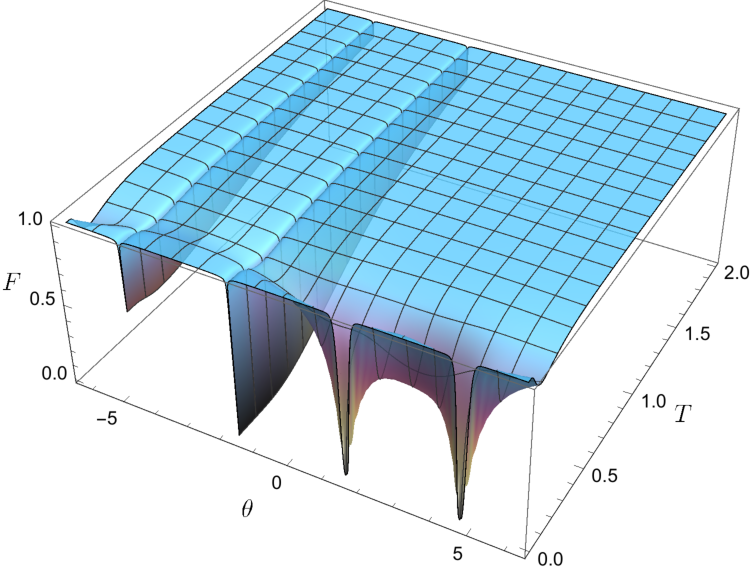
\includegraphics[width=0.20\textwidth,height=0.15\textwidth]{plot3}
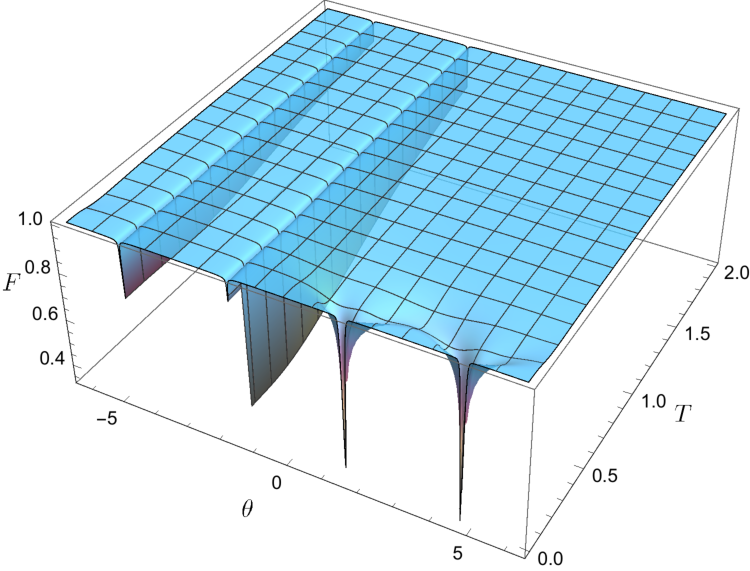
\includegraphics[width=0.20\textwidth,height=0.15\textwidth]{plot4}
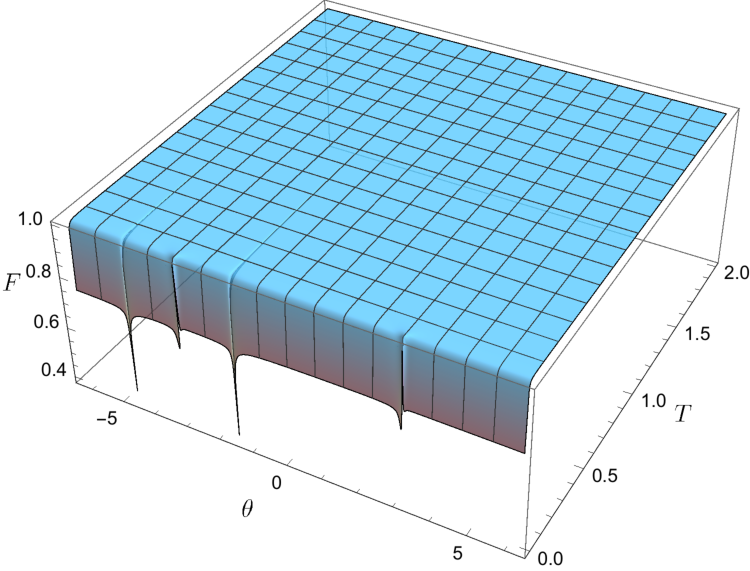
\includegraphics[width=0.20\textwidth,height=0.15\textwidth]{plot1}
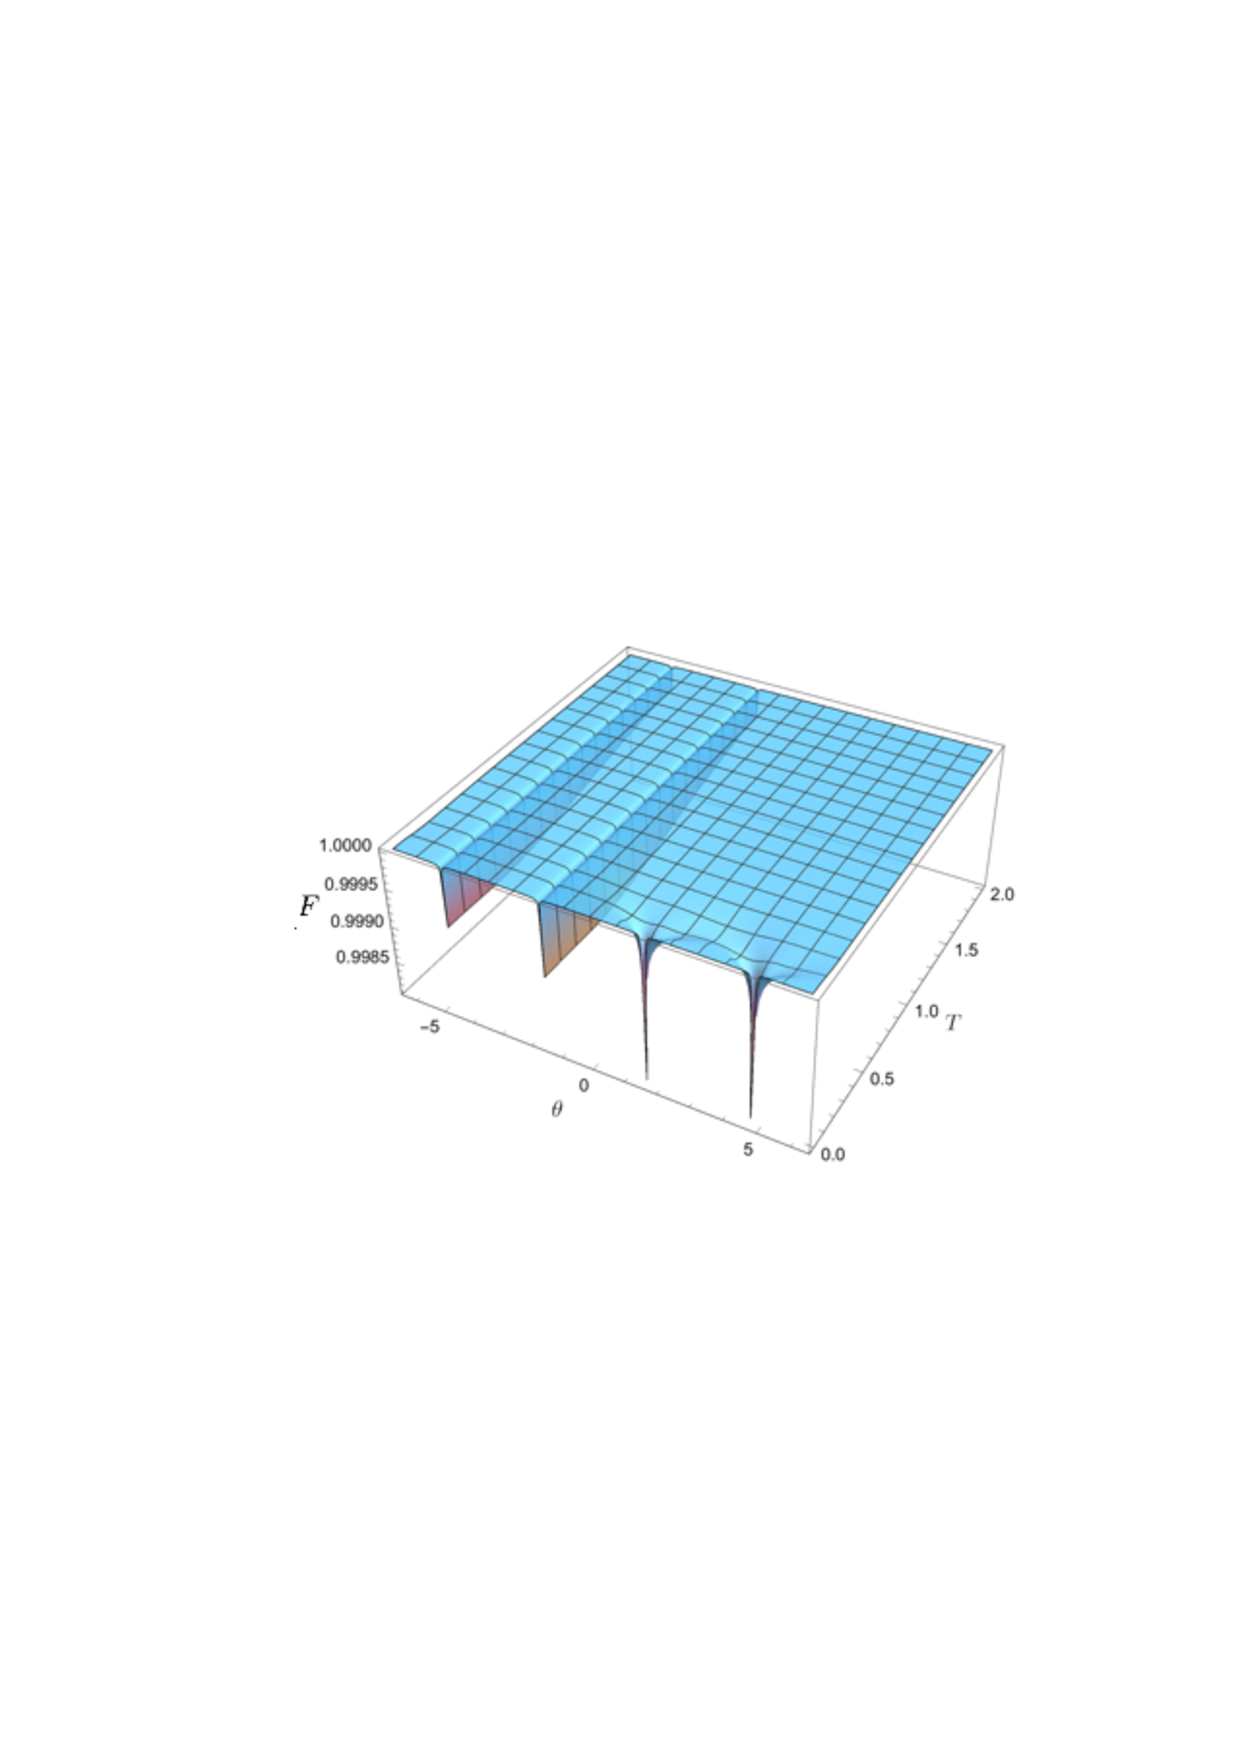
\includegraphics[width=0.20\textwidth,height=0.15\textwidth]{plot2}
\end{flushleft}
\end{minipage}
\begin{minipage}{1.22\textwidth}
\begin{flushleft}
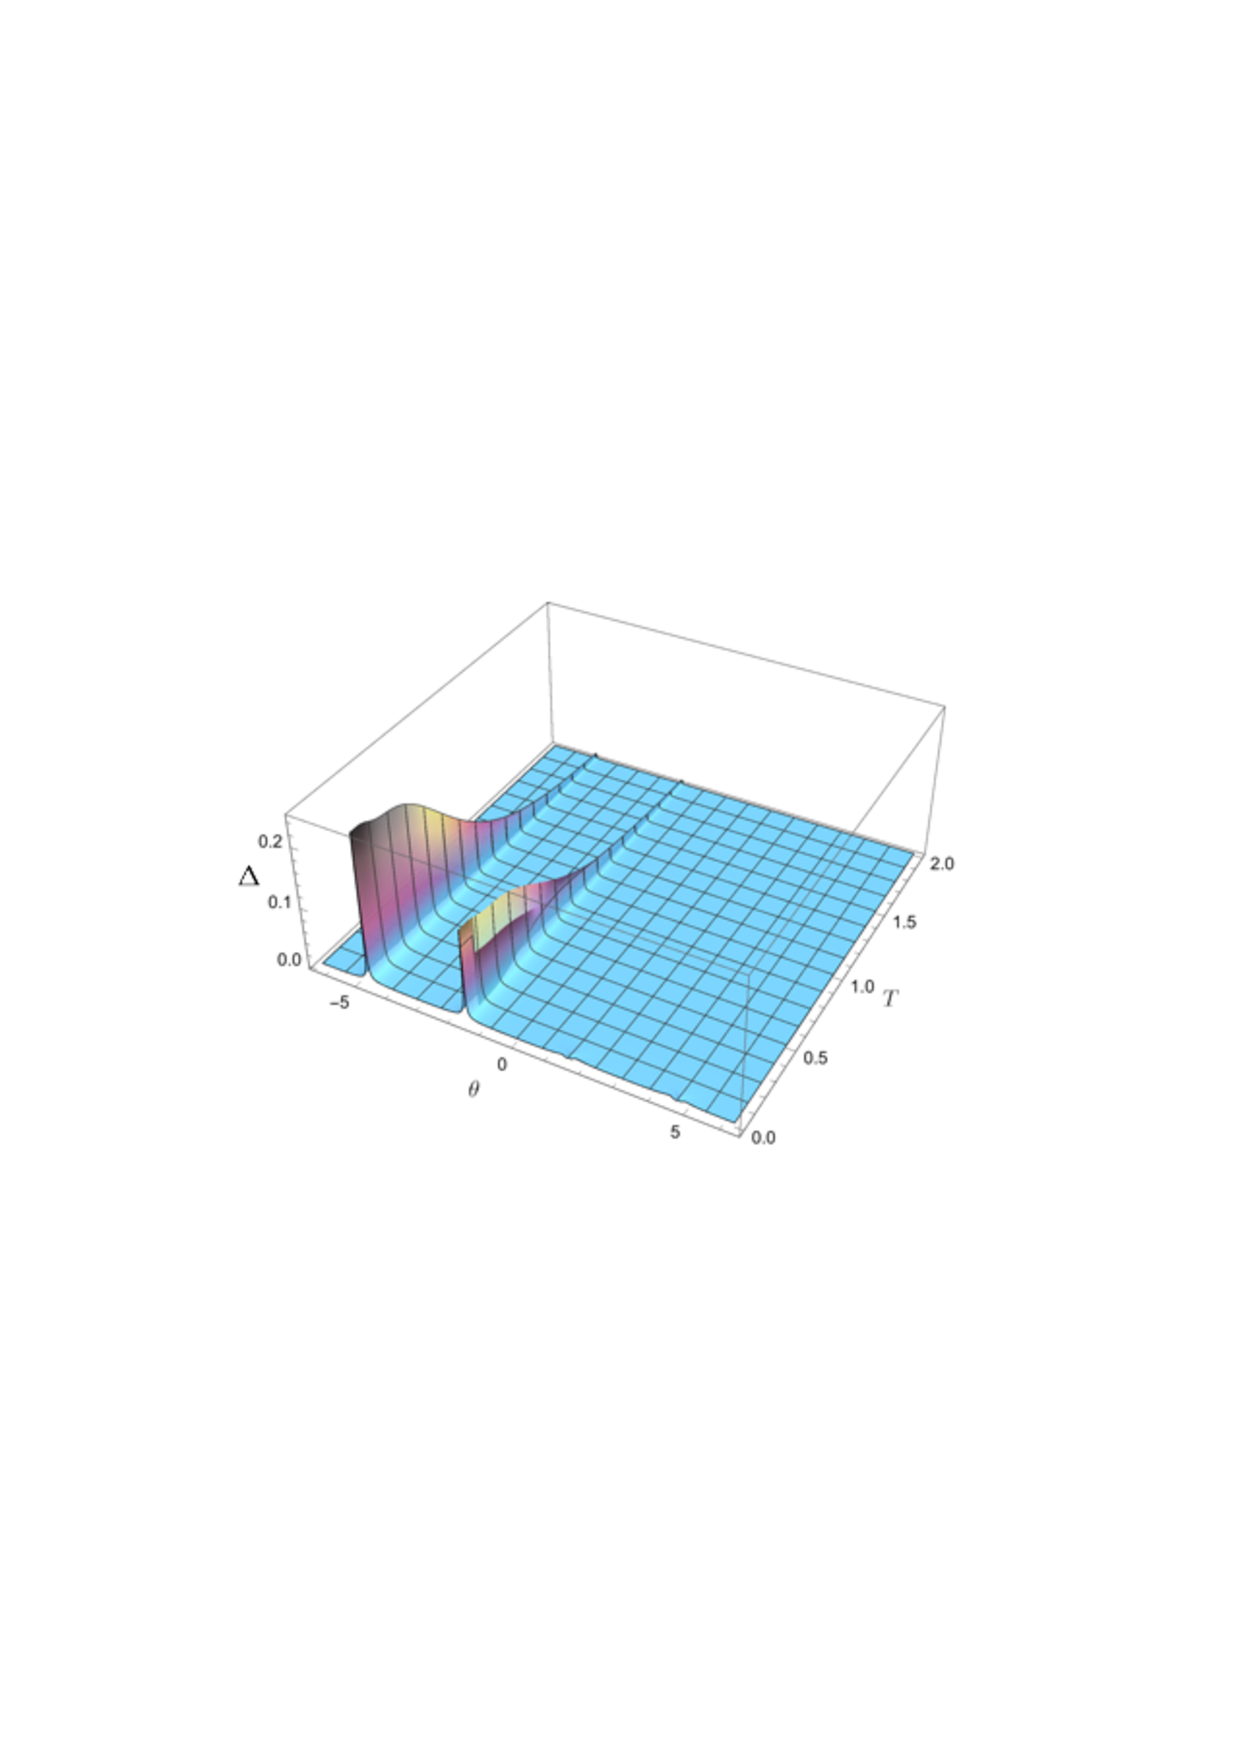
\includegraphics[width=0.20\textwidth,height=0.15\textwidth]{plot7}
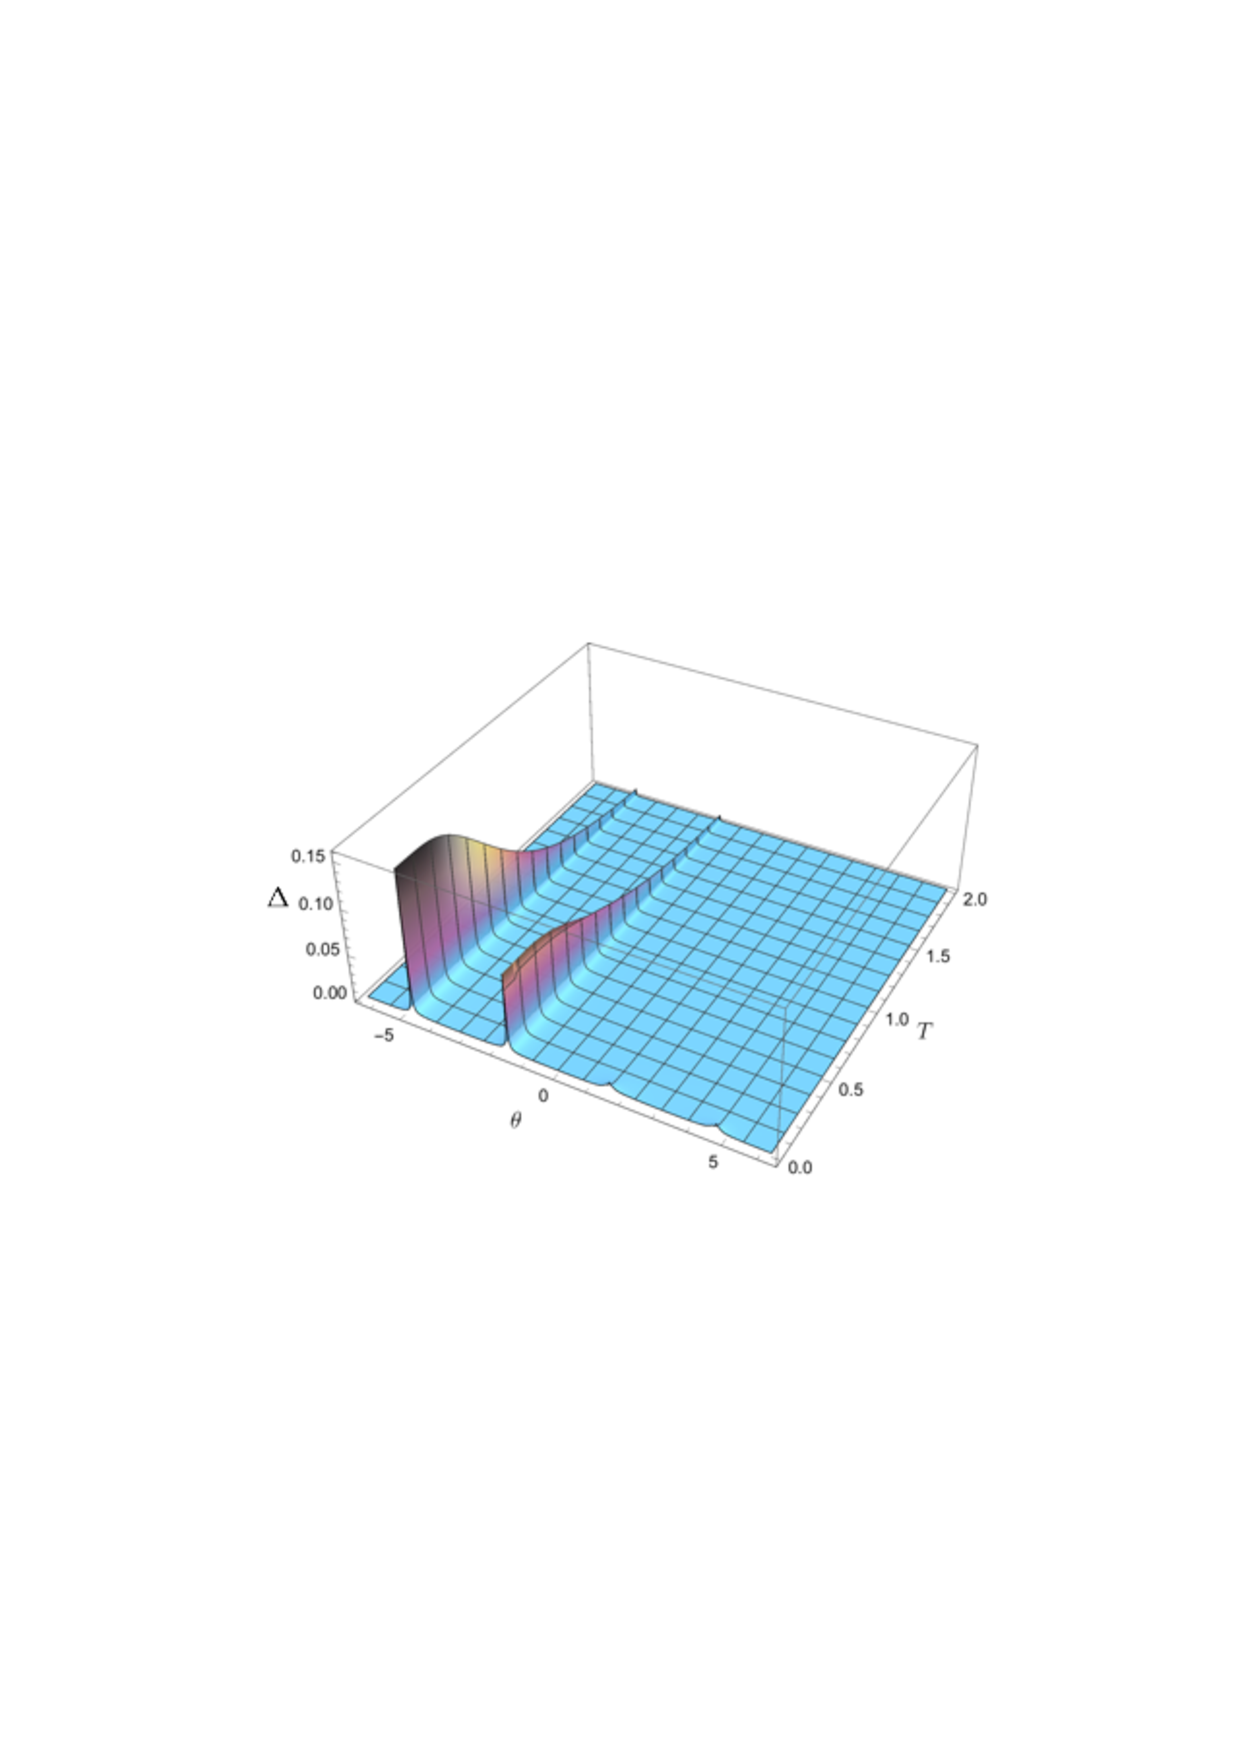
\includegraphics[width=0.20\textwidth,height=0.15\textwidth]{plot8}
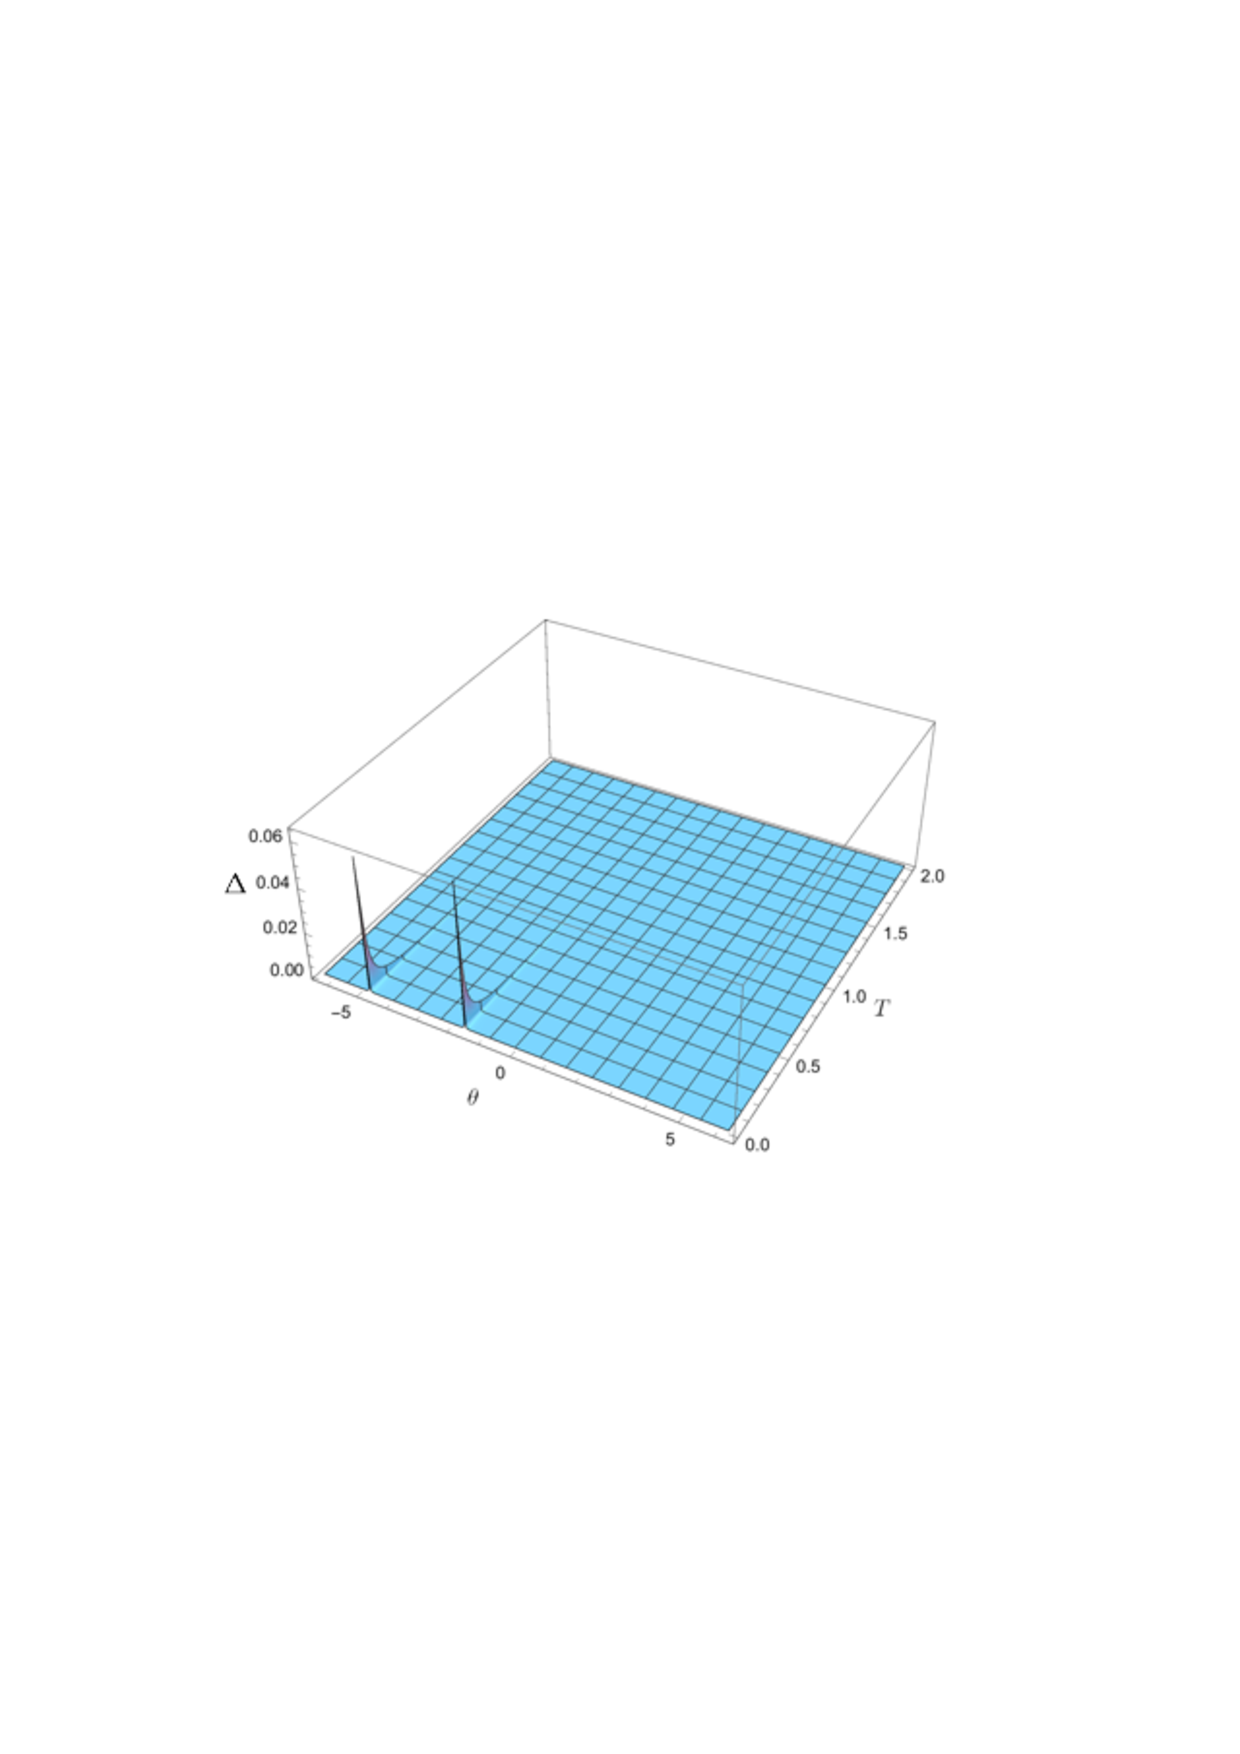
\includegraphics[width=0.20\textwidth,height=0.15\textwidth]{plot5}
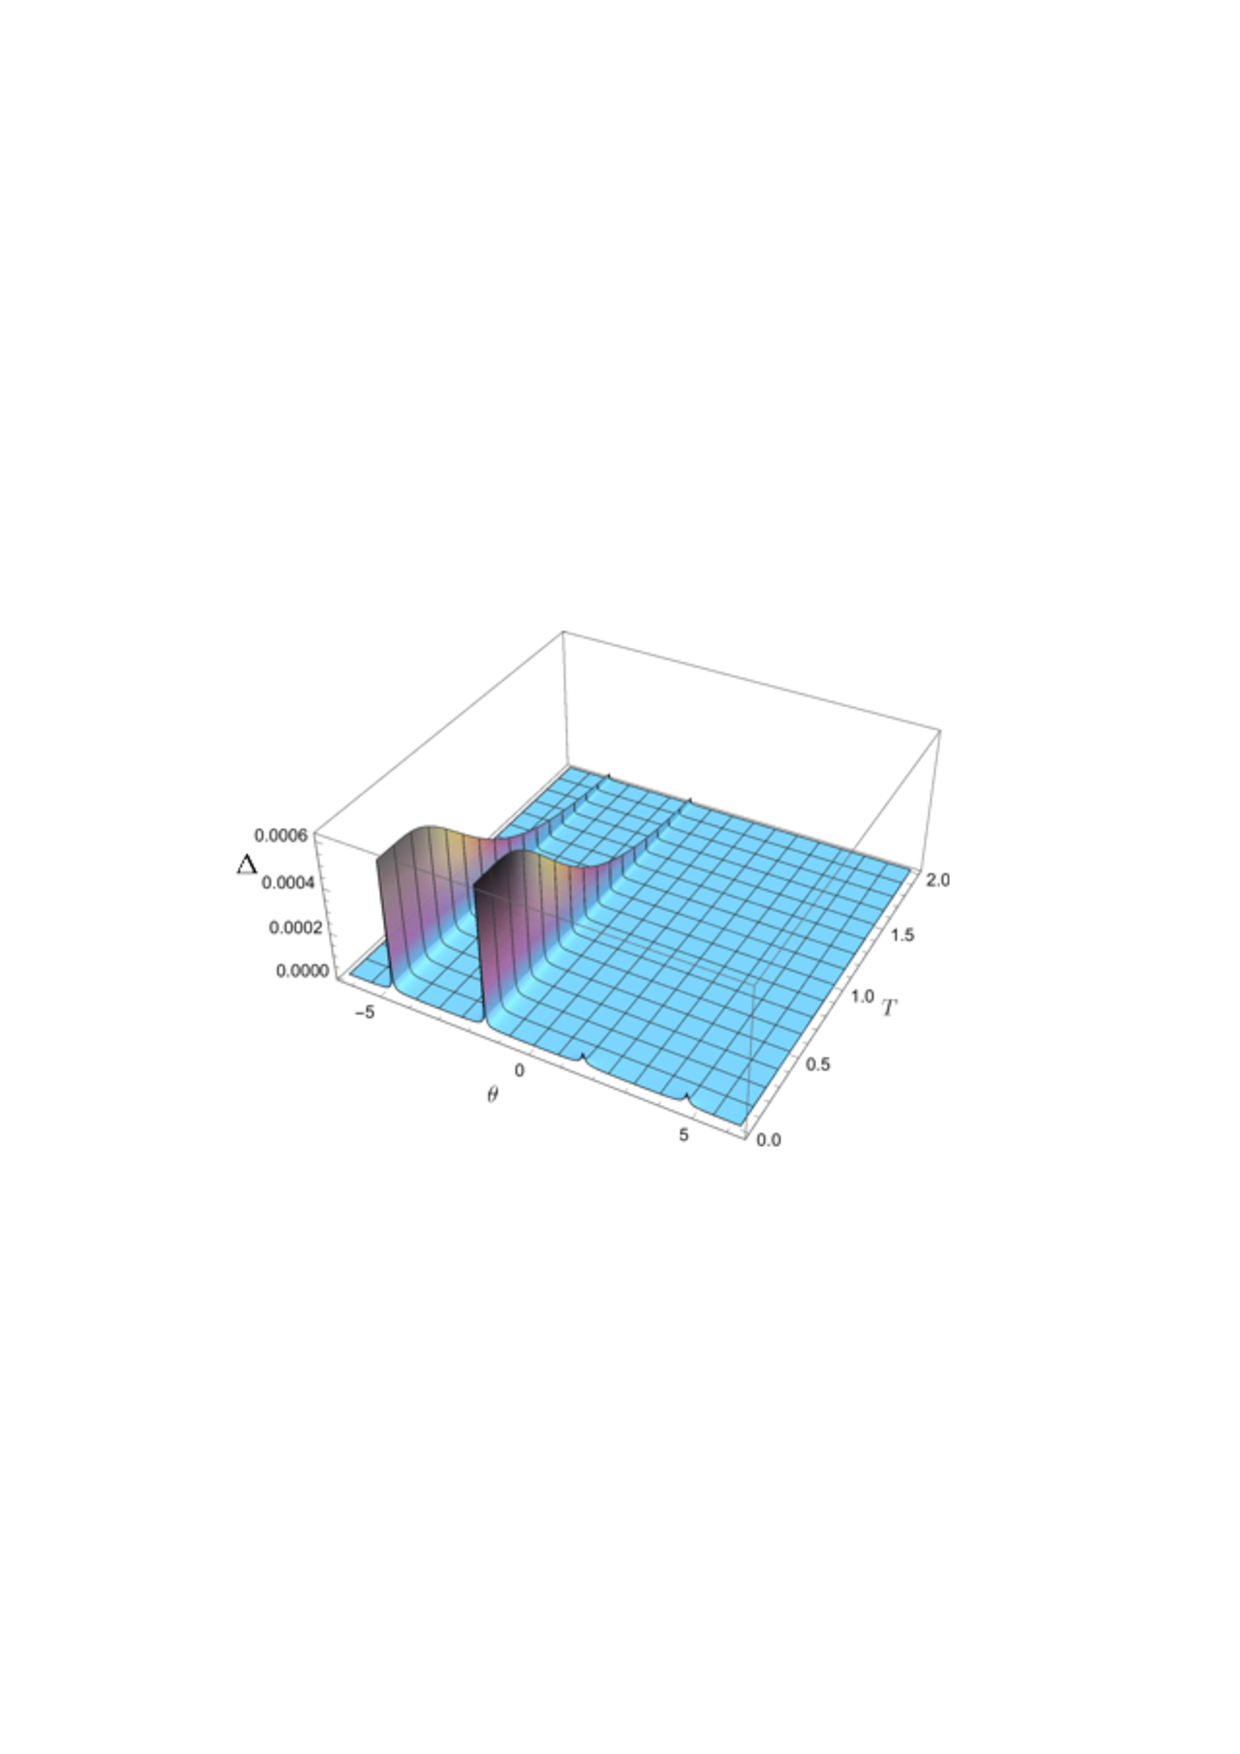
\includegraphics[width=0.20\textwidth,height=0.15\textwidth]{plot6}
\end{flushleft}
\end{minipage}
\begin{minipage}{1\textwidth}	
\caption{Fidelity (top) and $\Delta$ (bottom) for the many-body states $\varrho^{(0)}$ (left) and $\varrho^{(1)}$ (middle-left) and the single-particle states $\rho^{(0)}$ (middle-right) and $\rho^{(1)}$ (right), for the BDI symmetry class. $\delta \theta =\theta'-\theta=0.01$ and $\delta T=T'-T=0.01$. The small step in the top middle-left plot is due to numerical instability.}
\label{fig:fidelityBDI}
\end{minipage}
\end{figure}

\begin{figure}[h!]
\center
\begin{minipage}{1.22\textwidth}
\begin{flushleft}
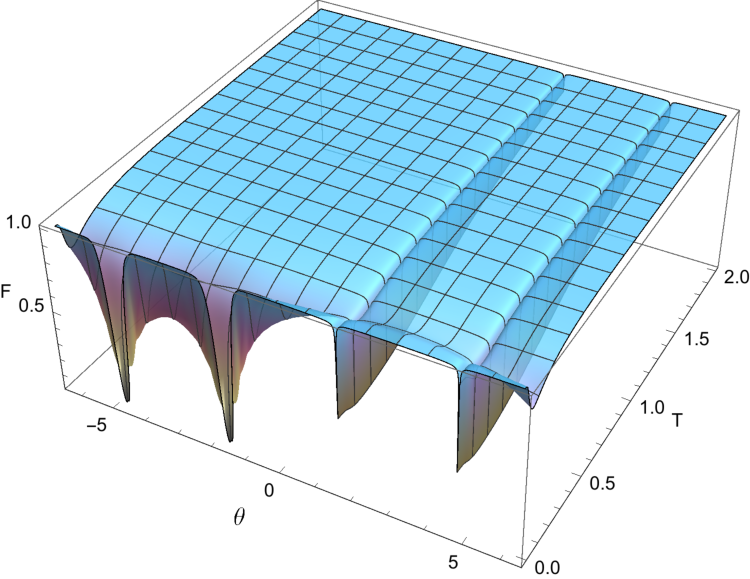
\includegraphics[width=0.20\textwidth,height=0.15\textwidth]{a3fidm0}
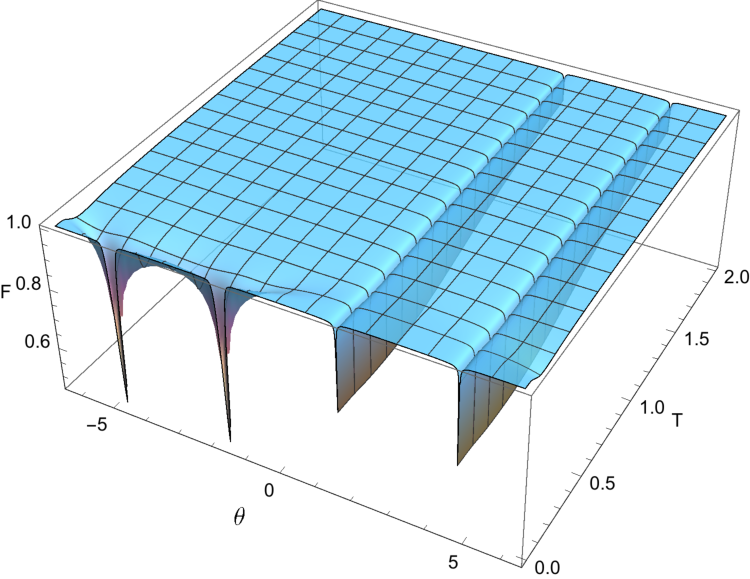
\includegraphics[width=0.20\textwidth,height=0.15\textwidth]{a3fidm1}
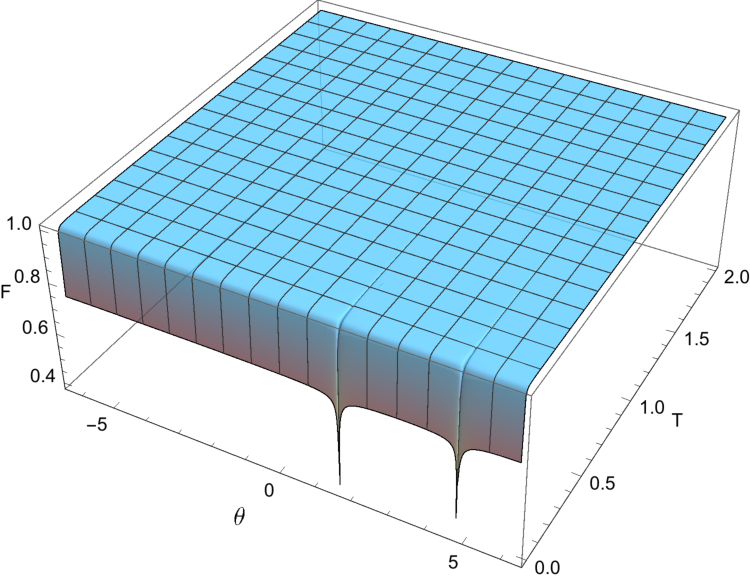
\includegraphics[width=0.20\textwidth,height=0.15\textwidth]{a3fids0}
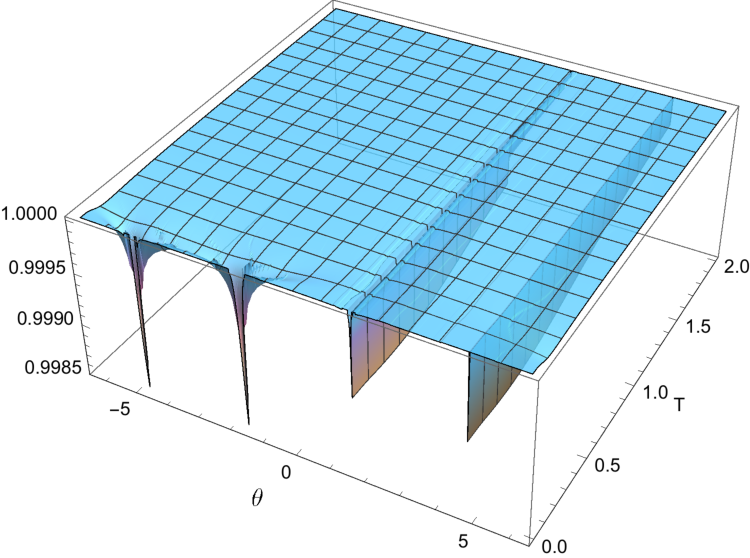
\includegraphics[width=0.20\textwidth,height=0.15\textwidth]{a3fids1}
\end{flushleft}
\end{minipage}
\begin{minipage}{1.22\textwidth}
\begin{flushleft}
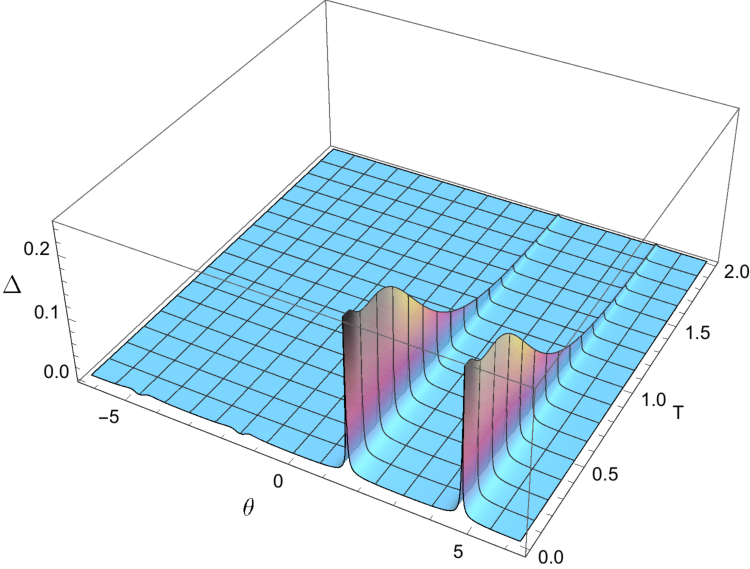
\includegraphics[width=0.20\textwidth,height=0.15\textwidth]{a3uhlm0}
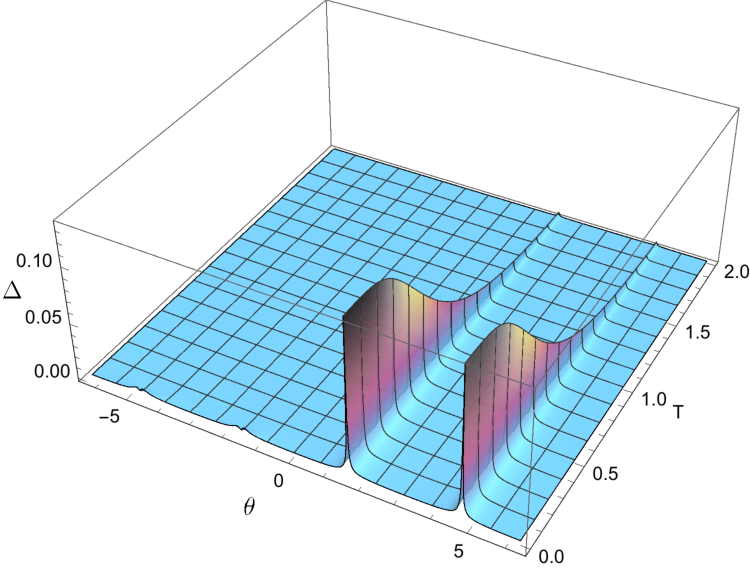
\includegraphics[width=0.20\textwidth,height=0.15\textwidth]{a3uhlm1}
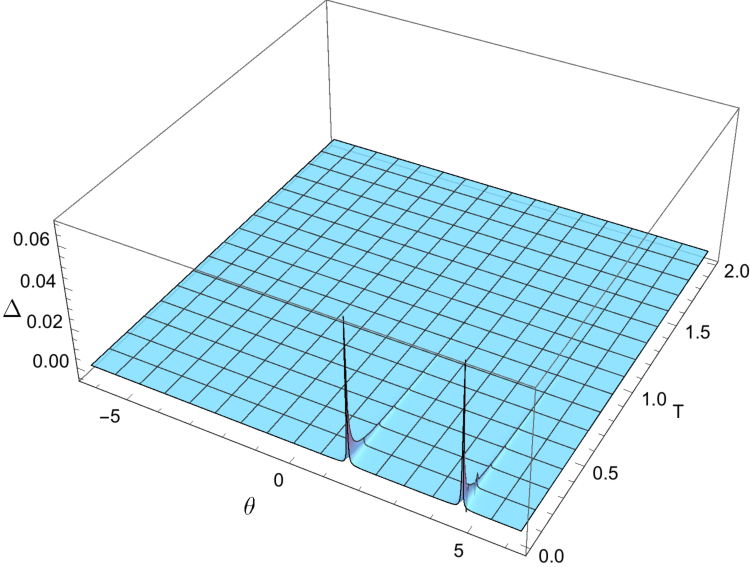
\includegraphics[width=0.20\textwidth,height=0.15\textwidth]{a3uhls0}
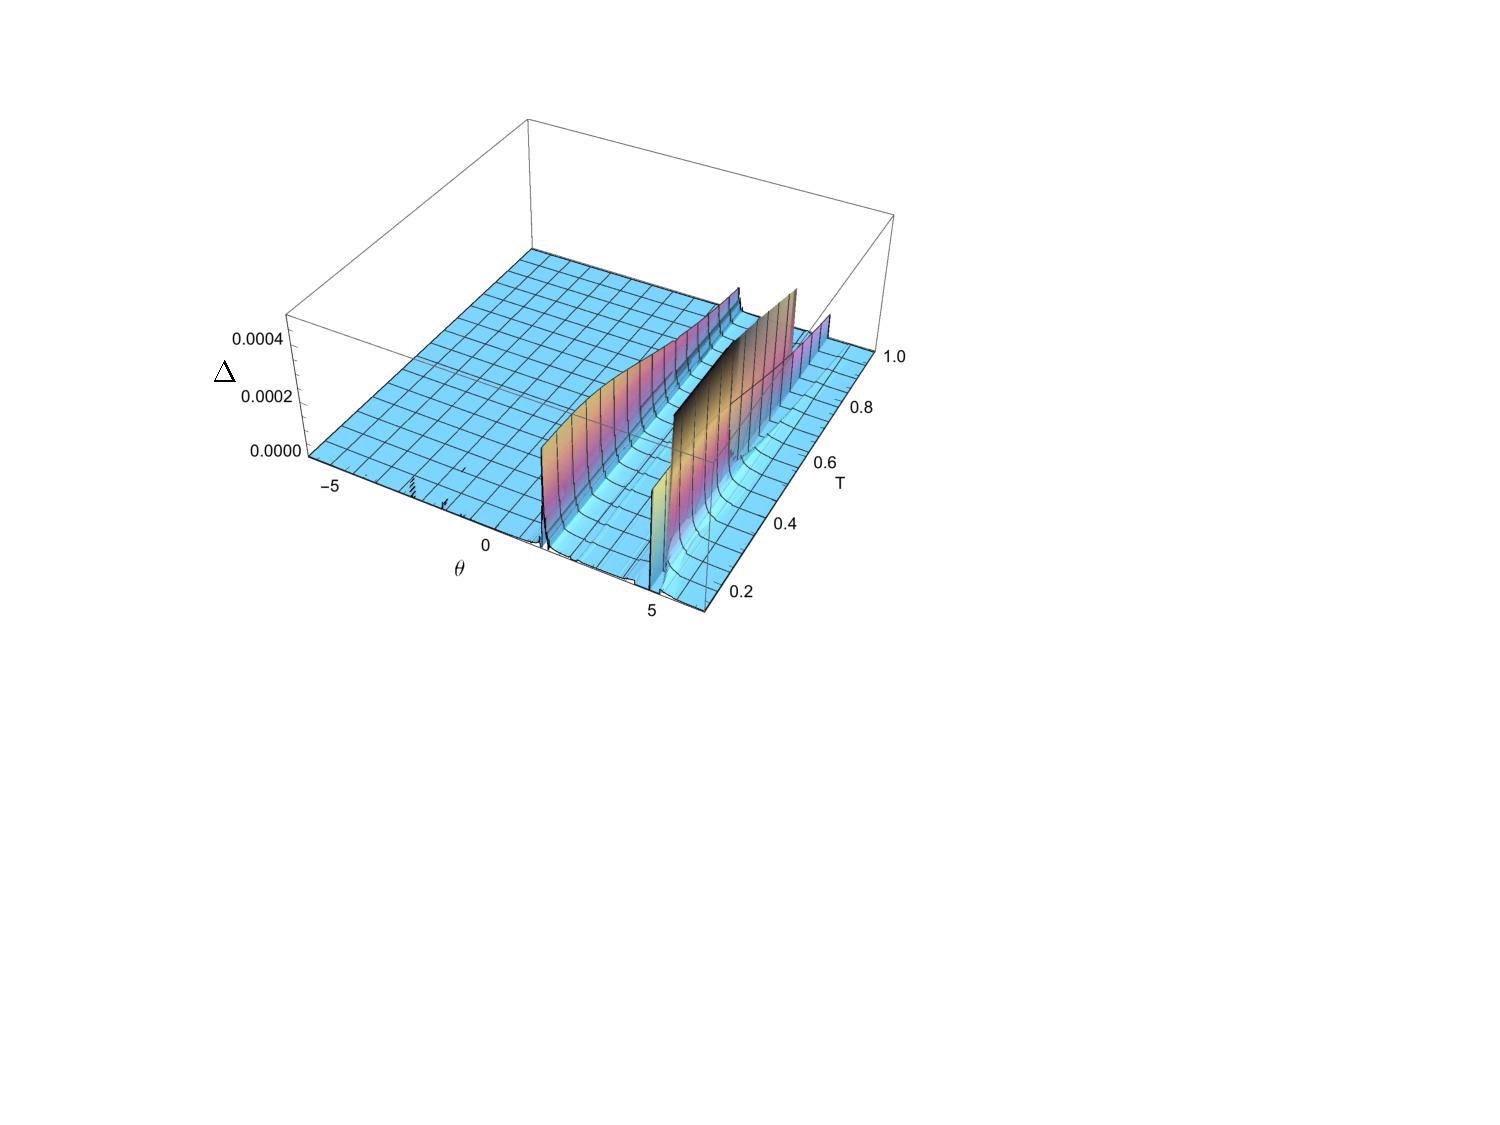
\includegraphics[width=0.20\textwidth,height=0.15\textwidth]{a3uhls1}
\end{flushleft}
\end{minipage}
\begin{minipage}{1\textwidth}	
\caption{Fidelity (top) and $\Delta$ (bottom) for the many-body states $\varrho^{(0)}$ (left)  and $\varrho^{(1)}$ (middle-left), and the single-particle states $\rho^{(0)}$ (middle-right) and $\rho^{(1)}$ (right), for the AIII symmetry class. $\delta \theta =\theta'-\theta=0.01$ and $\delta T=T'-T=0.01$. In the case of the state $\rho^{(1)}$, the quantity $\Delta$ is highly oscillating for temperatures close to $0$ in the neighbourhood of the critical points, therefore we show the results for a range of temperatures where these numerical instabilities are less prominent.}
\label{fig:fidelityAIII}
\end{minipage}
\end{figure}


A unique feature of periodically driven systems and their corresponding effective Hamiltonians is that both energies $E_k = 0$ and $E_k = \pi$ correspond to a closed gap (the difference between the two energy levels $\pm E_k$ becomes zero modulo $2\pi$). This special feature of QWs yields a surprising result in our analysis. In our study, we observe a different behaviour of the gap closing points with temperature, depending on whether they correspond to $E_k = 0$ (the two points with $\theta > 0$) or $E_k = \pi$ energy (the two points with $\theta < 0$). 
 Whenever the gap closes, the vector $\vec{n}_k(\theta)$ is ill-defined, but the behaviour of $F$ and $\Delta$ will be different due to their dependence on the entire energy spectrum. For the case of $E_k = 0$, they signal two isolated zero-temperature points of quantum PTs, corresponding to $\theta = \pi /2,\ 3\pi /2$ (in the case of $\Delta$ we notice small, but still present, peaks at these points). As the temperature increases, they are no longer signalling a PT and this is due to the dependence on the hyperbolic sine of $E_k$, which vanishes for $E_k=0$ (see the respective formulae), thus eliminating the $\vec {n}_k\cdot \vec {n}'_k$ term carrying the relevant topological features. The significance of these points of the zero-temperature quantum PTs on the system in the low-temperature regime, and the existence of possible crossovers, remain as open questions and require further investigation. In contrast to that, for the $E_k=\pi$ gap closing points, the PT lines survive with temperature, hence revealing a ``finite-temperature quantum PT'' (a PT occurring at finite temperature, driven solely by the Hamiltonian's parameter(s), and not the temperature). Again, this can be understood through the dependence on $E_k$ via hyperbolic functions which take finite values for $E_k=\pi$, thus maintaining the dependence on $\vec{n}_k\cdot\vec{n}'_k$.
 
 Notice that for $\rho^{(0)}$ the qualitative behaviour is different from the other three types of states: the fidelity does not drop for $T=0$ and $\theta = \pi /2, 3\pi /2$, while it does for two new $T=0$ points at $\theta = \pm\pi$. The first difference is due to the fact that the zero temperature limit of $\rho^{(0)}$ projects only onto $M$ given by the points of minimum energy $-E_k=-\pi$, see Equation~\eqref{eq:rho0_lim}. Thus, both quantities do not see the critical momentum at which the gap closes at zero energy, which is above the lowest mode. The abrupt change of the fidelity at the points where $\theta=\pm \pi$ is the consequence of the enhanced zero-temperature ground state distinguishability due to the fact that $E_k$ becomes constant and independent of $k$, i.e.,  the zero-temperature state projects onto the whole Brillouin zone ($M(\theta = \pm\pi) = \mathcal B$). Notice also that in the respective plot for $\Delta$, the absence of peaks at $\theta = \pm\pi$ is consistent with the fact that the Uhlmann factor quantifies the change of eigenvectors, while the presence of two peaks at the corresponding fidelity plot is due to the flattening of the spectrum, i.e., solely to the change of eigenvalues. Observe that while the results for the representatives of BDI and AIII classes are qualitatively similar, the zero-temperature fidelity corresponding to the $\rho^{(0)}$ states for the AIII representative only exhibits drops in the gap closing points ($-E_k=-\pi$), as the spectrum is always non-trivially $k$-dependent.
 
Let us now comment on the results for the fidelity and the quantity $\Delta$, in the case where we probe the system with respect to the parameter of the Hamiltonian and the temperature, separately. In the first case, where $\delta\theta=0.01$ and $\delta T=0$ ($\delta\vec{q}=(0.01,0)$), the results are qualitatively the same as the ones presented in Figures~\ref{fig:fidelityBDI} and~\ref{fig:fidelityAIII} for $\delta\vec{q}=(0.01,0.01).$ In the second case, where we probe the system only with respect to temperature, that is $\delta\theta=0, \delta T=0.01$ or more concisely $\delta\vec{q}=(0,0.01),$ the results for the fidelity are qualitatively the same as the ones for $\delta\vec{q}=(0.01,0.01),$ while the results for the quantity $\Delta$ are different. In particular, we obtain that $\Delta$ is equal to zero everywhere. This triviality is due to the fact that $\Delta$ quantifies the difference between the eigenbases of $\rho$ and $\rho'$, as mentioned before and in this case that we only change the temperature and not the parameter of the Hamiltonian, the eigenbasis remains the same. On the other hand, the fidelity drops at the points of the PT, since it is also sensitive to changes in the spectrum. Notice that the results for these two cases are in agreement with the results presented in the previous Chapter 4, which were also obtained by separately probing the system with respect to the temperature and the Hamiltonian parameter.
\section{The edge states} 
\label{sec:edgeqw}
We proceed to our study of the edge states. The bulk-to-boundary correspondence principle~\cite{x:g:wen:91,ryu:hat:02} predicts their existence on the boundary between distinct topological phases. These states are symmetry protected, i.e., they are robust against perturbations of the Hamiltonian which respect the symmetries of the system. In the case of pure states, QWs realise the aforementioned principle as shown in~\cite{kit:rud:ber:dem:10,kit:12}. In particular, the authors made $\theta$ change along the line, as 
$\theta(x) = \theta^{(t)}H(x_0-x) + \theta^{(n)}H(x-x_0)$, where $H(x-x_0)$ is the Heaviside step function and $\theta^{(t/n)}$ are the values of the angle for the trivial/non-trivial phase, respectively. This way, they were able to create a phase boundary at the site $x_0$ of the line, where $\theta$ changes. The edge states are then observed by evolving the walk \textit{in time} from the initial state localised at the phase boundary: the probability to find the system in the initial position keeps being (considerably) higher than for the rest of the line, due to the overlap between the initial state with the edge state that is localised there.

In our case, we are interested in probing the robustness of the edge states with respect to temperature. Therefore, we study an ensemble of the BG type which corresponds to a stationary state of the split-step QWs realising the BDI and AIII class representatives, with the position-dependent coin operation, parameterised by its temperature $\beta^{-1}$. This stationary state appears naturally if one looks at the von Neumann evolution equation for the density matrix and imposes the stationarity condition. By diagonalising $H_{\text{eff}}$ we obtain the localised states which can either have quasienergy $0 \text{ or }\pi$. Here, we choose a different order for the energy spectrum, by promoting the edge states with energies $E=\pi$ and $E = 0$ to be ground states, so that they survive at the zero-temperature limit. 

\begin{figure}[h!]
\center
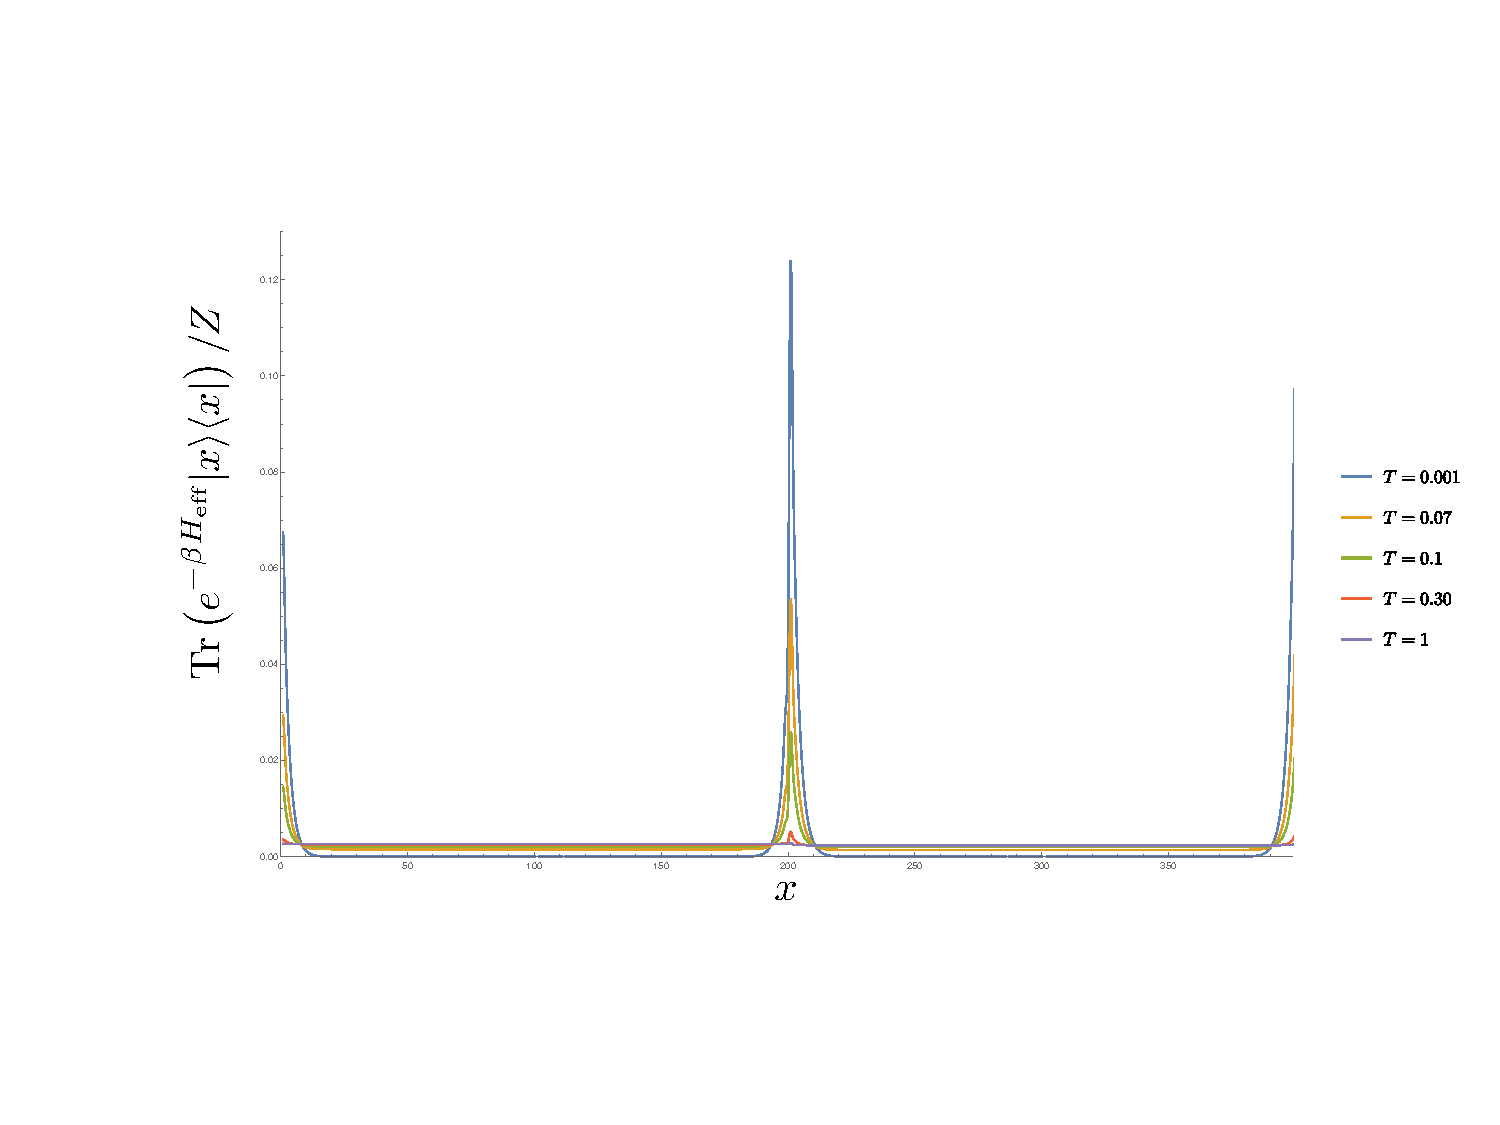
\includegraphics[scale=0.4]{edgestates_BDI}
\caption{
Position probability distribution of the QW simulating the representative of the BDI class, as a function of the sites, $\tr (e^{-H/T}\ket{x}\bra{x})/Z$. The Hamiltonian $H$ is obtained by varying $\theta$ along $x$ through a step-like function~\cite{kit:rud:ber:dem:10}. The domain wall is centred in the middle of the line. Periodic boundary conditions are taken, hence the edge state at the boundary.}
\label{fig:edgeBDI}
\end{figure}

\begin{figure}[h!]
\center
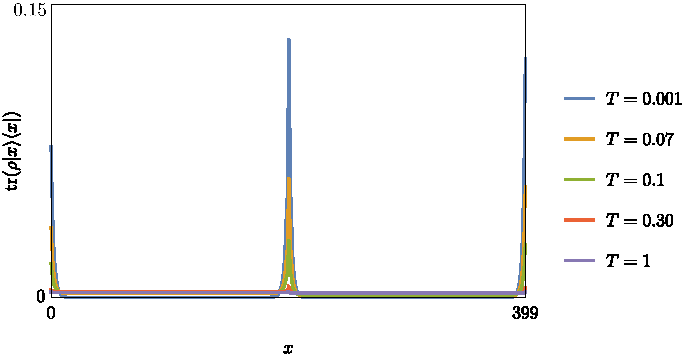
\includegraphics[width=0.6\textwidth,height=0.25\textwidth]{plot9.pdf}
\caption{Position probability distribution of the QW simulating the representative of the AIII class, as a function of the sites, $\tr (e^{-H/T}\ket{x}\bra{x})/Z$. Again, the parameter $\theta$ of the Hamiltonian, changes along $x$ according to a step-like function~\cite{kit:rud:ber:dem:10}. The boundary  is centred in the middle of the line and periodic boundary conditions are taken.}
\label{fig:edgeAIII}
\end{figure}


We observe that at $T=0$, the edge state has the major contribution to the probability distribution. As temperature increases, the edge states are smeared out, see Figure~\ref{fig:edgeBDI} for the BDI class representative and Figure~\ref{fig:edgeAIII} for the representative of the class AIII. Since the presence of an edge state is a clear manifestation of the topological order at $T=0$, the fact that it does not disappear for higher temperatures, but it is rather smeared out, suggests that the topological nature of the system is preserved in agreement with the fidelity and $\Delta$ analysis for the $E_k=\pi$ gap-closing points.

Our fidelity and $\Delta$ analysis revealed that for $T>0$ there exist no thermal PTs (i.e., no temperature-driven PTs), as also shown in Chapter 4 for paradigmatic models of TIs and TSCs. However, here we observe finite temperature \emph{parameter}-driven PTs. The non-existence of thermal PTs is further confirmed by the behaviour of the edge states, which are gradually smeared out as temperature increases, as also pointed out in~\cite{viy:riv:del:14}. Note that the edge states studied here are probed through a different method from the one used in Chapter 4. There, a small chemical potential was introduced in such a way that the zero-temperature behaviour of the many-body density operator is the projector onto the Fermi sea. Consequently, the existence of the edge states was signalled by the abrupt change in the number operator on the sites where they appeared.





\section{Conclusions}
\label{Conclusions and Outlook}
We derived analytic expressions for the fidelity and the quantity $\Delta$ between two BG states for QW representatives of topological phases for the chiral symmetric classes BDI and AIII and their many-body counterparts. For the systems considered, the fidelity is detecting the points where the Bloch vector is ill-defined, which corresponds to the closure of the gap. Since in our case the phase diagram is such that the closure of the gap always means the change from a trivial phase to a nontrivial one, and vice versa, the fidelity is capturing the topological PT. Our results show the absence of temperature-driven PTs in two ways: through the fidelity analysis and through the behaviour of the edge states appearing on the phase boundary. In addition, the analysis of the fidelity and, through the quantity $\Delta$, the Uhlmann connection shows the existence of finite-temperature PTs driven solely by the Hamiltonian's parameter $\theta$. We would also like to point out that, providing that one of the goals of this study is to investigate the finite-temperature behaviour of topological order in realistic many-body systems, the fact that the behaviour of the single-particle BG states is consistent with that of their many-body counterparts, shows that the analysis of the former can be a useful mathematical tool in the study of the latter.

Finally, we would like to point out some possible future lines of research. First, the same study could be applied to the rest of the symmetry classes in 1D and 2D using the protocols introduced in~\cite{kit:rud:ber:dem:10}. Further analysis of realistic noise effects that can give rise to these BG states, in particular the single-particle ones, presents another interesting line of research (for a partial answer to this question, see also a recent study of the effects of thermal noise onto single-particle factor states of a topological insulator~\cite{riv:viy:del:13}). The above study could also be conducted for 2D QWs, as well as in the realm of multi-particle QWs.\\



%
%
%\bibliography{bibforthesis}
%\bibliographystyle{unsrt}
%
%\end{document}
